\section{Exoplanetary Context}\label{sec:ch1_context}

    Over the last three decades, the plethora of exoplanetary system detections has revolutionized the way we understand how planetary systems form and evolve. Since the discovery of the first extrasolar planets (exoplanet) around a main-sequence star, (HD~114762~b and 51~Pegasi~b \textbf{reference}), a revolution has occurred in our understanding of planetary formation and evolution. We have seen exoplanets of a variety of flavors; gas giants at fractions of an astronomical unit (AU) from their star, binary planetary systems, compact multi-planet systems. Giant planets are found with eccentricities ranging from 0--0.9, with sometimes large mutual inclinations. And roughly 50\% of solar type stars have a chance of hosting a compact multi-planet system with periods shorter than a year \textbf{see Review by Winn \& Fabrycky 2015}. 
    
    In contrast, in our Solar System, the planets follow nearly circular, low inclination orbits at distances that separate terrestrial and gas giants (see \S~\textbf{Section on Solar System}). Of course there are a few exoplanetary systems that may seem architecturally similar to our own. The HR~8799 multi-planet system is the perfect example, where its four directly imaged giant planets are at the same distance from the HR8799 star as our Jovian planets are, scaled to the Luminosity of our Sun \textbf{Reference and/or image}. 
    
    
    However, a number of questions arise if we try to place the origin of our Solar System in context to the diversity of exoplanetary systems:  differences between the Solar System and what we have observed around other stars leads to a number of questions. Can we truly understand the diversity of planetary systems? Is the existence of another habitable planet likely? If so, how can we identify such systems?
    %===================================================================
    %                DIVERSITY OF EXOPLANETS
    %===================================================================
    \begin{figure}
    \centering
    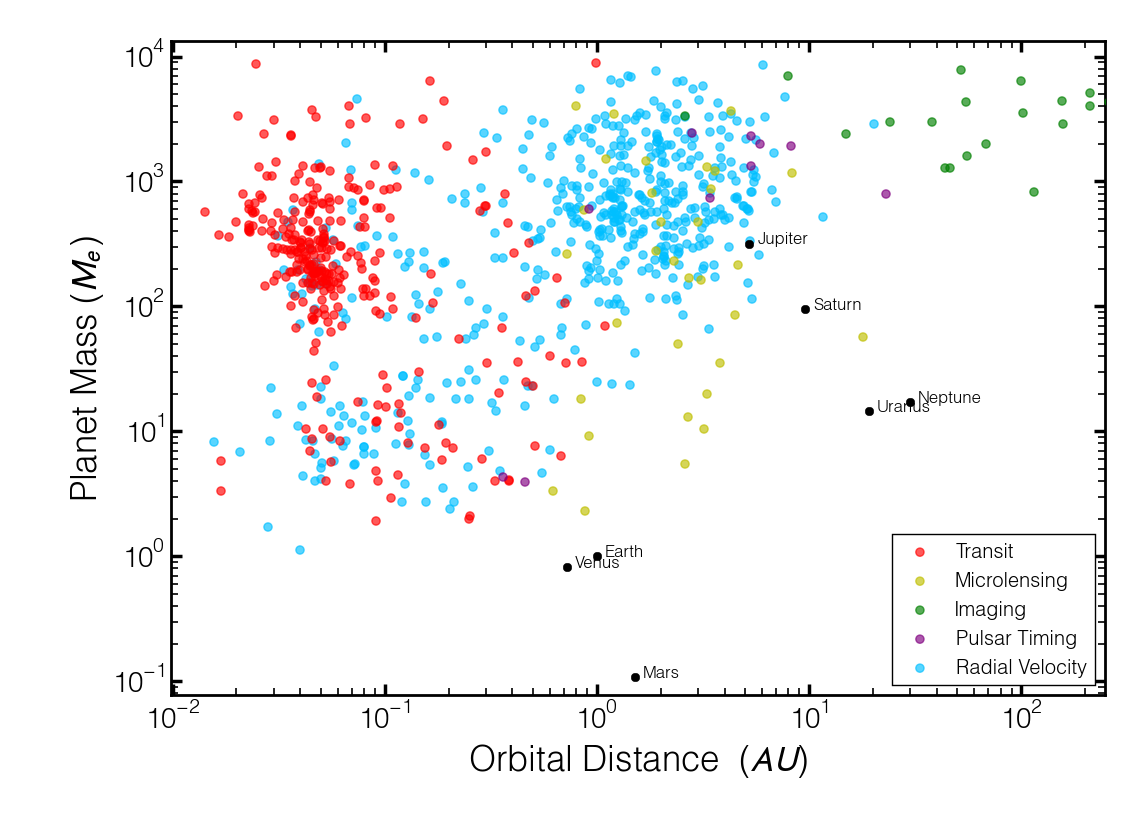
\includegraphics[scale=0.6]{Ch1/exoplanet_detections_june2015} 
    \caption[Exoplanet Statistics]{Not representative of all plaents -- those that don't have distances are not plotted. Mix of msini and m listed.}
    \label{fig:known_exoplanets}
    \end{figure}
    %===================================================================
    
    Since the template of our Solar System is a requirement to address the above questions, it is fitting to investigate the Solar System in greater detail. One aspect of our Solar System that can be used to place its origin and evolution in context is via the circumsolar debris disk. Given that our own debris disk is created from the interplay between the planets and the minor bodies, studying exo-debris disks can inform us of potentially undiscovered planetary systems, as well as help place our own Solar System in context. Thus, the next question to ask is whether nature can mimic a similar disk architecture such as ours and how we our system fits into the backdrop of the multitude of planetary system detections. 
    
    This thesis takes a step toward answering such profound questions by identifying additional systems which have previously been overlooked and may hold a wealth of information in terms of...
    
    
    
\section{The Solar System's Debris Disk}\label{sec:ch1_ssdisk}

     \subsection{Current Configuration}
    
    Since I will be discussing debris disk detections motivated by the need to place our Solar System in context, it only makes sense to discuss in some detail our own Solar System's planetary system. The eight planets in the Solar System are follow a rather orderly configuration. The orbits are close to circular ($<0.21$), and are closely inclined to the invariable plane, ranging from $0.33^{\circ}$--$2.19^{\circ}$. The latter fact applies to all the planets except for Mercury, which has an inclination of $6.3^{\circ}$. The four rocky planets are located interior to 1.7~AU, while the four gas giant planets are located beyond the snow-line -- the point in relation to the Sun beyond which volatile molecules (e.g.,$H_20, CH_4$) condense -- all the way out to 30~AU. 
    
    %===================================================================
    %                  THE SOLAR SYSTEM DIAGRAM
    %===================================================================
    %\begin{figure}
    %\centering
    %\includegraphics[scale=0.6]{Ch1/???} 
    %\caption{Caption}
    %\label{fig:solar_system}
    %\end{figure}
    %===================================================================
    
    
    
    The inner and outer planets are also segregated by a physical barrier known as the Asteroid belt. Located between the orbit of Mars and Jupiter, the Asteroid belt spans a width of XX~AU and is composed of over a million kilometer-sized \textbf{check fact} objects that can be metallic, stony or even carbon rich in composition. In recent studies, some asteroids, such as $24 Themis$, have been found to be covered by an water-ice mantle \textbf{Campins2010-Nature reference}. It has been estimated that the mass of the Asteroid belt is XX Mearths, a value that was much larger in the early Solar System (see \S~\textbf{Section on Dynamics of SOlar system volution}. Beyond the orbit of Neptune lies a large reservoir or minor planets composed of icy, volatile, cometary material with sizes greater than XX. These minor bodies, distributed in a thin belt the width of XX~AU, are known as the Edge-Worth Kuiper Belt (EKB). \textbf{Maybe give a reference for a larger review?}.
    
    %===================================================================
    %               THE Zodiacal Dust 
    %===================================================================
    \begin{figure}
    \centering
    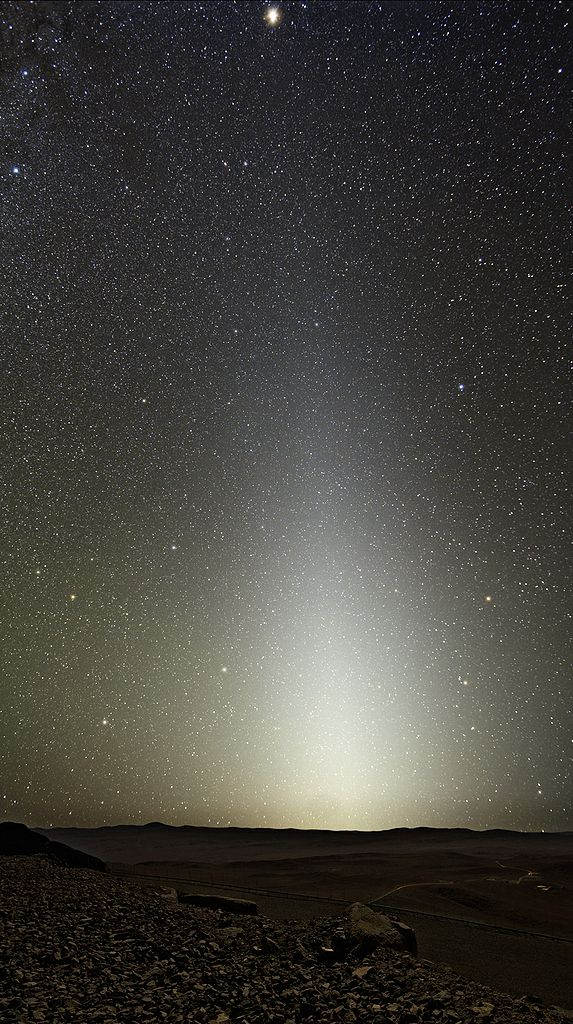
\includegraphics[scale=0.95]{Ch1/Zodiacal_Light_Paranal} 
    \caption[Zodiacal Light On Earth]{Zodiacal Light by ESO. Reference to ZD picture http://www.eso.org/public/unitedkingdom/images/zodiacal-light/}
    \label{fig:ZD_ESO}
    \end{figure}
    %===================================================================
    
    
    
    In addition to the rings of large rocky bodies, a disk composed of 10--100$\mu m$ sized cometary and silicate grains inhabits the Solar System. This disk, known as the Zodiacal Cloud, has been seen in scattered light observations (Hahn+2002), thermal emission (Kelsall+1998, Maris+2006) from the \textit{Infrared Astronomical Satellite} (Sykes 1990), the \textit{Spitzer Space Telescope} (Reach 2007) and others, as well as from spacecraft impact experiments. From the ground, the Zodiacal Cloud can be seen only on the darkest of skies, as a faint glow along the ecliptic (see Figure~\textbf{Figure of ZD}). The inner Zodiacal Cloud extends from the orbit of Venus all the way out to Jupiter. From most recent studies, namely \citet{Nesvorny2010}, the small particles which comprise the disk are thought to be mainly created from the grinding down of mm--cm sized grains, whihc themselves are ejected by spontaneous disruption from Jupiter Family Comets (JFC) as they approach the large tidal forces of Jupiter's gravity. The overall mass of the inner Zodiacal Cloud has been estimated to be $\sim1-2\times10^{19}$~g. To place this number into perspective, the bolometric Luminosity of the disk compared to that of the Sun is $L_{ZODY}/L_\odot \sim 2\times10^{-7}$. 


    
    \subsection{Dynamical Evolution Of Our Planetary System}
    
    Beyond just learning about the structure of the present-day Solar System, it is important to understand how the Solar System evolved into what we see now. This is for many reasons, but mainly because it is the only system where we know life exists. Although it is impossible to detail the entire history of the Solar System's evolution, it is important to understand that the current architecture of the Solar System would not be possible without the combined evolution of the planets as well as the remnant asteroidal and cometary disks. 
    
    It is generally accepted that the planets formed within the first 100 Myr (upper limit based on the final accretion to create Earth \citep{Allegre2008}), after the Sun reached its place on the main-sequence. During this time, it is thought that the planets were in a more compact configuration, within 15~AU \citep{Batygnin  Brown 2010}. Roughly 4.0--3.7 Gyr ago, scattering of the planetismal populations that lay outside the orbit of Neptune at 15~AU resulted in angular momentum exchange between the Gas Giants and the disk. This led to a period of instability, in which Jupiter and Saturn's orbits diverged, eventually crossing their mutal 1:2 mean motion resonance. From this, Jupiter migrated inward by $<0.5$~AU \citep{Mordibelli2010}, and pushed Saturn, Uranus and Neptune further out into the Solar System \citep{Tsiganis2005}. 
    
    This migration led to a period known as the Late Heavy Bombardment (LHB). During this time, Jupiter's short migration would have depleted the Asteroid belt by a factor or 10, and 97\% of the EKB was probably removed as a result of Neptune's outward migration. The scattered comets and asteroids during this period are most likely responsible for the Lunar craters \citep{Gomes2005}. However, it is also thought that the majority of Earth's water supply was transported during the LHB either from the EKB or from water rich asteroids. In addition, the depletion of the Asteroid belt by Jupiter has implications for the emergence of life on Earth, as a massive Asteroid belt today would imply a higher frequency of Terrestrial impacts. 
    
    \textbf{Some last sentence/paragraph on just one example and that w/o the disk, perhaps the planets would not be where they are, and Earth may not have the necessary resources to allow life to flourish. Also add in a line about how we would like to witness this type of evolution around other stars to place the SS in context.}
    
    %LHB lasted between 10 and 150 Myr
    %various resonance structures now in SS (Jupiter and AB, Neptune and KB)
    
      % Due to the gravitational influence of Jupiter, a number of (resonances)


%INSERT FIGURE OF ZD BRIGHTNESS DISTRIBUTION FROM NESVORNY 2010 (Fig 17.


\section{Circumstellar Disk Evolution}
    
    To understand something something in context of solar system, 
    The majority of disks are detected from the excess radiation in the infrared at levels greater than expected from the stellar photosphere (i.e., infrared excess), which arises from the heating of gas and dust in in the circumstellar environment. A detailed discussion of this will be in \S~\textbf{section on debris disk detections}


    \subsection{Protoplanetary Disk Phase}
    
    The paradigm of planet formation begins with a nascent protoplanetary disk (PPD), with primordial gas and dust that remains post-star formation, and which is then used to build the planets that we have detected. The primordial material forms into a circumstellar disk, as a consequence of angular momentum conservation. and is heavily sensitive to the angular rotation of the central star ($\Omega^2$) and even more sensitive to the infall time of the primordial material ($t_{infall}^3$) \citep{Terebey1984}. It is well accepted that 90-99\% of a PPD, is composed of gas, with the rest in the form of mm to micron sized dust grains. The bulk of the gas is comprised of neutral $H_2$, and mid-IR rotational lines have been observed from hot ($>600$~K) $H_2$ from the ground in the AB~Aur system \citep{Bitner2007}. Typically, however, tracers such as $CO$, and $HCN$ line emissions are observed at sub-mm wavelengths to detect the gas in PPDs (e.g. for stars in young associations such as Ophiuchus \citep{Andre1994} and Taurus-Auriga \citep{Beckwith1990}). These type of observations have shown that the size of these disks can range from 10--100~AU, with masses $>0.005M_\odot$ \citep{Osterloh1995}. These dust masses are typically derived by excess fluxes at mm-wavelengths, with extrapolations of the spectral distribution by assuming an upper limit to the grain size (usually around mm sizes) and some assumed opacity values \citep{Beckwith1990}. 
    
    \textbf{I was writing this part of my thesis when New Horizon's crossed Pluto earlier in the day.}
    
    Within the first $\sim$10~Myr, the majority of the primordial gas and dust has been dissipated. Viscous accretion of gas and dust onto the star has been attributed to the clearing of the inner regions (a few AU) of the star, which is supported by a lack of near-IR flux (2--5$\mu m$) and the presence of forbidden line accretion signatures \citep[(e.g., O~I, S~II)][]{Hartigan1995}. Photoevaporation from the central star will also carve out the outer disk. In this process, high-energy UV and X-Ray photons can excite gas and dust molecules enough so that they are no longer bound to the system, and simply evaporate into interstellar space. The replenishment of material into the inner disk after accretion halts is inhibited from extreme-UV photons from the central star. 
    
    
    During this entire process, grain-growth becomes important, as it not only removes mass from the gas rich, but also provides the seeds for future planetary creation. Small micron sized grains will typically feel a pressure gradient, since the gas rotates at non-Keplerian speeds. From this, grains will eventually collide, increase in mass and size, and be dragged to the mid-plane of the disk, where they can further grow to form the cores of potential planets, as well as asteroids and comets. 
    
    
    
    Within the first few million years, the inner 5--10~AU is 
    
    
    
     
    
    
    
        
    \subsection{Debris Disk Phase}
    
    \subsubsection{Detecting and Characterizing a Debris Disk}


PPDs are optically thick and thus tend to remit much of the star light in the IR (fdgt1e-2)

PR- Drag (Burns 1979, Bertotti+2003)

    

    
\section{Debris Disk as Signposts for Planets}


\section{Thirty Years of Debris Disk Observations}












